\documentclass[oneside]{book}

% Load the VUB package.
% This has many options, please read the documentation at
% https://gitlab.com/rubdos/texlive-vub
\usepackage{vub}

%href package to make references clickable.
\usepackage{hyperref}
\hypersetup{
    colorlinks,
    citecolor=black,
    filecolor=black,
    linkcolor=black,
    urlcolor=black
}

% Used for abbrivations etc
\usepackage{glossaries}

% Some highly suggested packages, please read their manuals.
\usepackage{cleveref}
\usepackage[natbib,style=apa]{biblatex}
\addbibresource{../bibliography.bib}
\usepackage{listings}
\usepackage{wrapfig}


%smaller spacing
\usepackage{titlesec}
\titlespacing*\section{0pt}{12pt plus 4pt minus 2pt}{0pt plus 2pt minus 2pt}
\titlespacing*\subsection{0pt}{12pt plus 4pt minus 2pt}{0pt plus 2pt minus 2pt}
\titlespacing*\subsubsection{0pt}{12pt plus 4pt minus 2pt}{0pt plus 2pt minus 2pt}

%space between paragraph and indent all
\setlength{\parskip}{1em}
%\usepackage{indentfirst}



%quotes
\usepackage{epigraph}

%space between bib entries
\setlength\bibitemsep{2\itemsep}

%images settings
\graphicspath{ {./images/} }
\usepackage{graphicx,caption}
\usepackage{float}
\usepackage{rotating}
\usepackage{tikz}

% subfigures
\usepackage{subcaption}

% Math
\usepackage{amsmath,bm}
\usepackage{amsfonts}

% Code
\usepackage[linesnumbered,ruled,vlined]{algorithm2e}
\DontPrintSemicolon
\renewcommand{\KwSty}[1]{\textnormal{\textcolor{blue!90!black}{\ttfamily\bfseries #1}}\unskip}
\renewcommand{\ArgSty}[1]{\textnormal{\ttfamily #1}\unskip}
\SetKwComment{Comment}{\color{green!50!black}// }{}
\renewcommand{\CommentSty}[1]{\textnormal{\ttfamily\color{green!50!black}#1}\unskip}
\newcommand{\assign}{\leftarrow}
\newcommand{\var}{\texttt}
\newcommand{\FuncCall}[2]{\texttt{\bfseries #1(#2)}}
\SetKwProg{Function}{function}{}{}
\renewcommand{\ProgSty}[1]{\texttt{\bfseries #1}}

% remove chapter text
\usepackage{titlesec}

\titleformat{\chapter}[display]
  {\normalfont\huge\bfseries}{}{0pt}{\Huge}
\titlespacing*{\chapter}
  {0pt}{0pt}{15pt}

% Init glossary
\makenoidxglossaries

% Add glossary entries
% Add glossary entries
% ref glossary with \Gls{latex}
% ref acronym with \acrshort{bci} or \acrlong{bci}


%% ------- AI related -------
\newacronym{ai}{AI}{artificial intelligence}
\newacronym{ml}{ML}{machine learning}
\newacronym{rl}{RL}{reinforcement learning}
\newacronym{drl}{DRL}{deep reinforcement learning}
\newacronym{dl}{DL}{deep learning}
\newacronym[plural=ANNs,firstplural=artificial neural networks (ANNs)]{ann}{ANN}{artificial neural network}
\newacronym[plural=DNNs,firstplural=deep neural networks (ANNs)]{dnn}{DNN}{deep neural network}
\newacronym[plural=CNNs,firstplural=convolution neural networks (CNNs)]{cnn}{CNN}{convolution neural network}
\newacronym{mlp}{MLP}{multilayer perceptron}
\newacronym{marl}{MARL}{multi-agent reinforcement learning}

%% ------- general -------
\newacronym{irl}{IRL}{in real life}
\newacronym[plural=MDPs,firstplural=Markov decision processes (MDPs)]{mdp}{MDP}{Markov decision process}

%% ------- approaches -------
\newacronym{dp}{DP}{dynamic programming}
\newacronym{dqn}{DQN}{deep Q-network}

%START title
\title{RL IRL}
\subtitle{A feasibility study of using Reinforcement Learning for varying difficulty bots in simple Python games}
\author{Lennert Bontinck}
\date{June, 2021-2022}
\promotors{Student number: 0568702}
\faculty{Computer Science: AI}
\begin{document}
\frontmatter
\maketitle
%END title


%TOC
\tableofcontents
\mainmatter

%START MAIN
\chapter{Introduction}
\label{ch:intro}

This chapter addresses the main concepts of \gls{rl} and why \gls{rl} has become more popular.
In section \ref{sec:intro-approaches}, some important differences in the possible approaches for solving \gls{rl} problems are highlighted.
Afterwards, some of the classical \gls{rl} problems that are solved to benchmark new state-of-the-art algorithms are introduced.
Finally, the feasibility of using \gls{rl} \gls{irl} is discussed.

%------------------------------------

\section{The reinforcement learning problem}
\label{sec:intro-problem}

\gls{rl} is a special type of \gls{ml} where algorithms are used to take actions in an environment.
These algorithms are often referred to as agents which should learn a policy that maps the current state of the environment ($S_t$) to an action ($A_t$) that can be taken in that state of the environment.
Upon taking an action, or after completing a series of actions, a reward ($R_t$) is given to the agent in the form of a positive or negative numerical value and the environment state may be updated.
Through repeated trial-and-error interactions, experience is collected.
This experience can then be used by the agent to learn a policy which chooses the optimal action for a given state.
According to \citet{rl_intro_handbook}, it is this trial-and-error search combined with a potentially delayed reward which distinguishes \gls{rl} from other types of \gls{ml}.
A typical \gls{rl} cycle is visualised in Figure \ref{fig:intro_rl_cycle}.

\begin{figure}[ht]
    \centering
    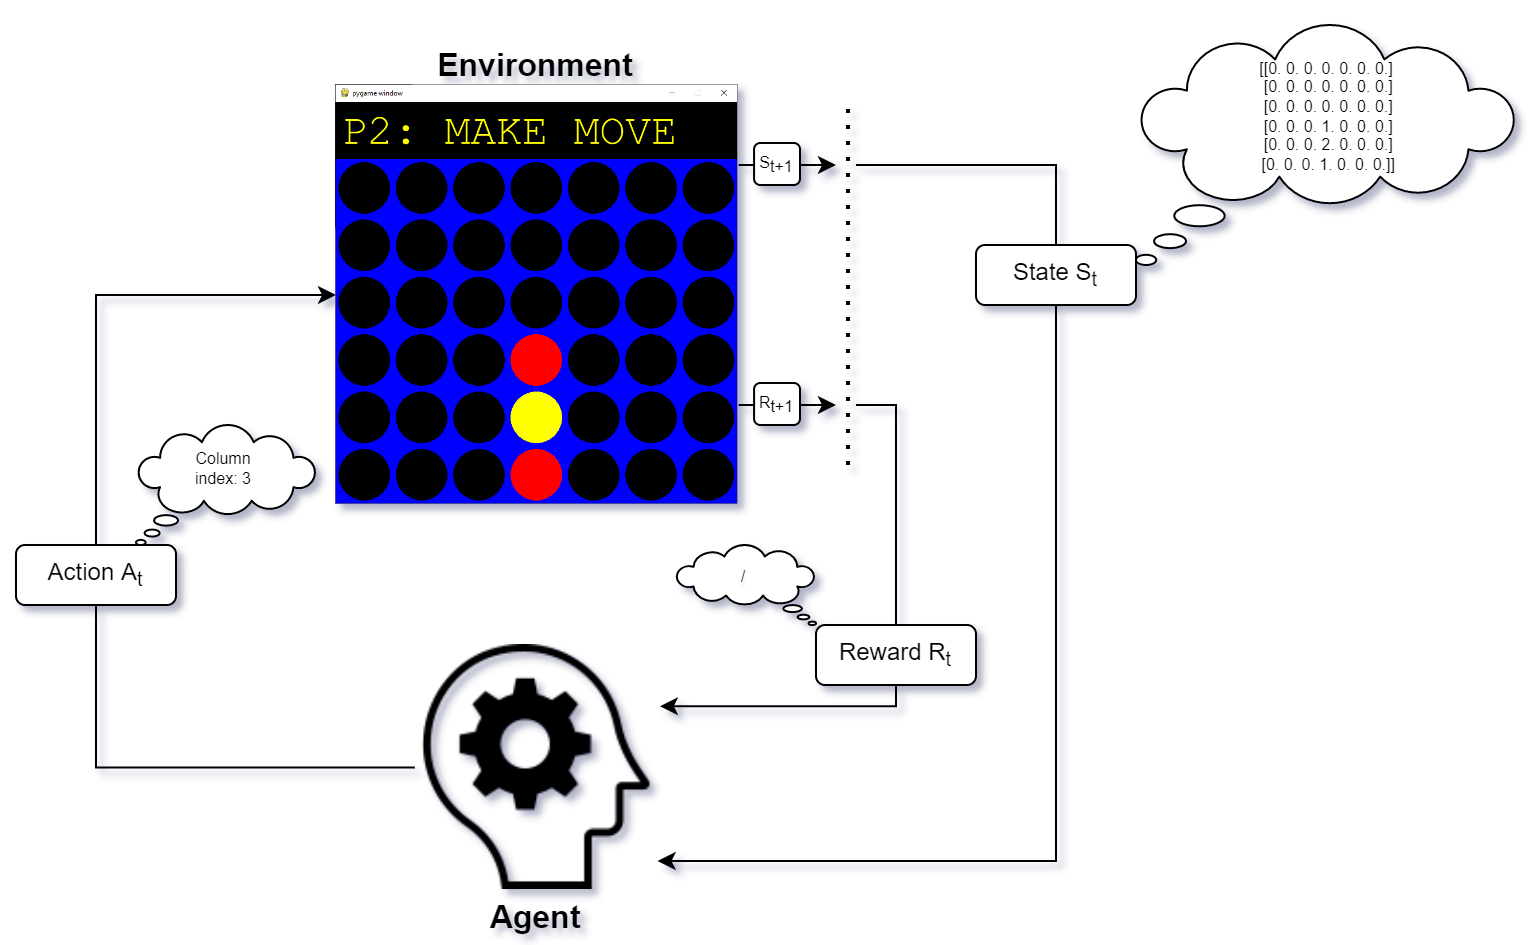
\includegraphics[width=0.9\linewidth]{images/rl_environment.png}
    \captionsetup{width=0.9\linewidth}
    \captionsetup{justification=centering}
    \caption{Typical \gls{rl} cycle annotated with examples for a single connect four game step which doesn't yield a reward.}
    \label{fig:intro_rl_cycle}
\end{figure}


Since the rewards can be considered a form of feedback given to the algorithm, these types of algorithms are not completely unsupervised.
However, classical supervised learning tasks often require far more supervision than \gls{rl}.
Consequently, \gls{rl} is often seen as a third \gls{ml} paradigm next to supervised and unsupervised learning.
Since the agent can learn in an online setting, there is also often no or minimal data needed upfront.
However, training an agent in an online manner, as to have the agent collect experience ($\approx$ data) itself, can take a considerable amount of time, even when using parallelized simulation.
It is also noted that offline \gls{rl} using pre-collected data for training exists.


As a result of not having direct instructions on what to do, it is difficult or even impossible for a \gls{rl} agent to decide if a learned policy is indeed the optimal policy.
Thus, an algorithm should be exploratory enough to evaluate many or even all possible policies over time whilst also being greedy enough so that the collected reward is being maximised according to the currently used policy.
Balancing this exploration/exploitation behaviour is one of many challenges in \gls{rl}.
A classical approach to solve this problem is by using epsilon-greedy.
In epsilon-greedy, epsilon ($\epsilon$) denotes the probability of taking a random action over the greedy action for any given step ($t$).
Finding a balance between exploration/exploitation becomes even harder when taking into account the time it can take to perform a singular step.
This means that mathematical proofs of optimal convergence for exploration strategies relying on infinite steps are even less likely to hold in real-life situations with finite time.

Whilst this definition of the \glsfirst{rl} problem remains rather abstract, it captures most of the requirements of a good \gls{rl} algorithm.
Indeed, the \gls{rl} problem is less concrete than some other problems in \gls{ml} allowing for high creativity in approaches.
Some of the many different types of approaches are discussed in section \ref{sec:intro-approaches}.
The handbook by \citet{rl_intro_handbook} gives a more detailed introduction to \gls{rl} if you have some form of computer science background.


%------------------------------------

\section{Markov Decision Process}
\label{sec:intro-mdp}

As discussed in section \ref{sec:intro-problem}, the \gls{rl} problem definition is rather abstract.
Whilst this allows for many types of solutions to be created, having a more formal representation of the \gls{rl} problem can be desired.
This is especially handy for mathematical reasoning over \gls{rl} and proving certain properties of a \gls{rl} algorithm.
To facilitate this need, \glspl{mdp} are often used as a mathematically idealized form of the \gls{rl} problem with specific properties.
Equation \ref{eq:intro_mdp} gives the mathematical definition of a \gls{mdp}.

\begin{equation}
\begin{aligned}
\text{MDP} &= \langle S, A, R, \gamma, p \rangle
\\
S &= \text{A set of states}
\\
A &= \text{A set of actions}
\\
R &= \text{A set of rewards}
\\
\gamma &= \text{A discount factor, } \gamma \in [0.1]
\\
p &= \text{A transition function which desribes the dynamics}
\end{aligned}
\label{eq:intro_mdp}
\end{equation}

Comparing the formal definition of an \gls{mdp} to the typical \gls{rl} cycle shown in Figure \ref{fig:intro_rl_cycle}, it becomes apparent that many of the \gls{rl} problems can indeed be formulated as a \gls{mdp}.
Many variants of \glspl{mdp} exist, with many of them often assuming certain properties such as the Markov property.
Intuitively, the Markov property means that the transition from the current state to the next state is only dependent on the current state and not on any of the previous states the agent was in.
For the annotated connect four example in Figure \ref{fig:intro_rl_cycle}, the Markov property holds.
Indeed, all aspects of the past agent-environment interaction that make a difference in the future are captured in the current state which is simply a representation of the board.
Intuitively, when neglecting potential human bias towards certain columns that could be learned, it doesn't matter how to current board emerged in deciding an optimal next move.
\citet{rl_intro_handbook} go over the Markov property and other properties that are often assumed for \glspl{mdp} in more detail.

As typical \gls{rl} problems can be represented as \glspl{mdp}, trying to solve \glspl{mdp} corresponds to solving the formalised \gls{rl} problems. Solving a \gls{mdp} corresponds to acting in the \gls{mdp} such that the expected discounted return is maximized.
The expected discounted return is given in Equation \ref{eq:intro_expected_discounted_return}.
From this equation, it becomes visible how important it is to choose a good discount factor since a low $\gamma$ will result in a \textit{myopic agent} ($\approx$ greedy) and a high $\gamma$ will result in a \textit{farsighted agent} ($\approx$ exploratory).
As a result, not only the reward influences the goal of a \gls{rl} agent but also the discount factor ($\gamma$).
It is noted that for some situations the discount factor can be 1, resulting in a special type of expected return: the undiscounted expected return.

\begin{equation}
G_t = R_{t+1} + \gamma R_{t+2} + \gamma^2 R_{t+3} + ... = \sum_{k=0}^{\infty}{\gamma^k R_{t+k+1}}
\label{eq:intro_expected_discounted_return}
\end{equation}


%------------------------------------

\section{Reinforcement learning is becoming more popular}
\label{sec:intro-popular}

The term \gls{ai} is used in conventional media a lot, even for systems that shouldn't be classified as \gls{ai}.
In contrast, terms like \gls{ml} are far less known by the wider public, let alone the term \gls{rl}.
However, the computer program that beat a world champion Go player is likely one of the most recent achievements of \gls{ai} the wider public will remember.
Indeed, with $\approx 10^{360}$ possible game states for the Go game, far bigger than $\approx 10^{123}$ for chess, the AlphaGo system by \citet{alphago} that beat a world champion Go player was a monumental milestone.
This AlphaGo system is a popular example of \gls{rl}, although the use of human and domain knowledge combined with provided known rules makes AlphaGo a non-pure form of \gls{rl}.
Follow up versions such as AlphaGo Zero \citep{alphago_zero}, AlphaZero \citep{alphazero} and MuZero \citep{muzero} focused on removing these extra dependencies from the algorithm, making them a purer form of \gls{rl} whilst also having better and more general performance. 

All of the above systems were created by DeepMind, a Google-owned company.
As the name of the company suggests, all of these systems combine \gls{dl} with \gls{rl} to create a special type of \gls{rl} often referred to as \gls{drl}.
Whilst \gls{dl} was revolutionising for many fields in \gls{ml}, it was especially groundbreaking in \gls{rl} research.
Indeed, whilst \gls{rl} has decades' worth of research coming from multiple almost independent threads of history \citep[Section 1.6]{rl_intro_handbook}, it was only with the introduction of \gls{drl} that the field has received high coverage in major publications journals such as Nature \citep{rl_intro_handbook, alphago, alphago_zero, dqn}.
Section \ref{sec:intro-approaches} explains in more detail why \gls{drl} is so powerful and how it opened many new doors for the \gls{rl} field.

When looking at the most impressive \gls{rl}-based systems, it becomes apparent that big companies and institutions such as DeepMind and OpenAI are responsible for the majority of these works.
Even state-of-the-art algorithms such as Rainbow by \citet[DeepMind]{rainbow} and famous libraries such as the Gym library by \citet[OpenAI]{gym} often originate from these bigger companies.
For newcomers first learning about \gls{rl} this may seem intimidating and raise the idea that \gls{rl} requires a lot of resources to create meaningful systems.
Whilst many examples can be given of extensions to existing algorithms and many libraries exist which are provided by smaller institutions or even individuals, complete systems from such smaller institutions with obvious real-life applications are harder to find.
Section \ref{sec:intro-irl} discusses the feasibility of developing such complete systems in more detail.

%------------------------------------

\section{Common approaches for reinforcement learning}
\label{sec:intro-approaches}

As discussed in section \ref{sec:intro-popular}, \gls{drl} has opened many new doors for the \gls{rl} field, but many more different approaches for \gls{rl} exist.
A first big division can be made on so called model-based and model-free approaches.
This differentiation relates to whether or not the algorithm requires a \textit{perfect model}.
Such a perfect model should give exact probabilities and information about all possible state-action pairs for an environment.
Whilst often used for proving theoretical aspects of \gls{rl} through \gls{dp}, these types of approaches don't have many other use cases.
This is in part because such a perfect model is in contrast with the ideology of \gls{rl} using delayed rewards.
More importantly, providing a perfect model has been proven to be computationally too hard or even impossible in most cases.
Contrary to what the name suggests, model-free approaches still require a model.
However, the model should only be able to generate experiences and thus fits in more easily with delayed rewards and is possible to be made in many more scenarios.
Take for example the simple game of connect four, a model that generates experiences by recognising a win, a loss or a tie is simple, allowing for model-free approaches.
Defining probabilities of each of these outcomes at any given state for any given action can become hard very fast, making model-based approaches impractical, if not impossible.
Section \ref{sec:connect_four_rl-harder_then_you_think} explains how connect four has over \textit{four trillion} possible board layouts ($\approx 10^{13}$), further illustrating how hard providing a perfect model can be.

Another major differentiation that is made between \gls{rl} algorithms is whether the algorithm is on-policy or off-policy.
As discussed in section \ref{sec:intro-problem}, the goal of an agent in \gls{rl} is to learn a policy which chooses an action for any given state.
This policy to be learned by the agent is called the \textit{target policy}.
This target policy is thus often the optimal policy, as we want the agent to learn to behave perfectly optimal in an environment.
However, for an agent to ensure that it is using the optimal policy, sufficient exploration of all possible policies should be done as was already discussed in section \ref{sec:intro-problem}.
Due to this balancing, a conflict of interest arises.
The requested agent's target policy is the optimal policy, but to ensure this, the agent has to remain exploratory causing it to never behave optimally the whole time.
Whilst strategies such as epsilon-decay exist, where the exploration is reduced over time to limit divergence from the optimal policy, these strategies are not always ideal.
What is essentially wanted is that the agent has a notion of two policies.
A \textit{target policy} which should be learned, e.g. the optimal policy, and a \textit{behaviour policy} to collect experience, e.g. the learned target policy that takes random actions systematically.
The relation between these two policies is what defines an algorithm to be on-policy or off-policy.
Off-policy indicates that both policies are different whilst on-policy indicates both policies are equal.
On-policy approaches can thus be seen as a special type of off-policy approaches.


A last important notion for this paper is \glsfirst{drl} approaches and how they differ from tabular approaches.
The main rationale behind tabular approaches is to maintain a big table of all possible states and the actions that can be taken in that state and associate a metric value to each such pair.
For example, each state-action pair might have an expected reward associated with it.
Choosing the action with the highest expected reward then boils down to choosing that state-action pair with the highest value and learning from experience consists of updating that table.
Whilst this can be very powerful for low complexity environments, it can quickly blow up in more complex environments.
Section \ref{sec:connect_four_rl-harder_then_you_think} discusses how making such a table for the relatively simple game of connect four can quickly become non-tractable.
\Gls{drl} doesn't maintain such a table but rather fits a deep learning model on the state and predicts actions from it.
This directly shows how \gls{drl} enables far more use-cases for \gls{rl}.
Since \gls{dl} is known to be great at reducing high-dimensional data such as images to low-dimensional features, it can also be faster to train for more complex environments that may still be viable to learn through tabular methods, although this is not always the case.
\Gls{rl} algorithms could be even further categorised based on other criteria and whilst these different categorisations are important, they fall outside the scope of this paper.


%------------------------------------

\section{Classical reinforcement learning problems}
\label{sec:intro-classical_rl}

A complete \glsfirst{rl} system consists of three main components: a conversion mechanism from an environment state to a computer representation of that state, a \gls{rl} algorithm that maps that environment state to an action and a component responsible for executing the chosen action.
In a real life environment system, these three different components often require a multi-disciplinary team to be implemented.
Take for example a \gls{rl} based robot lawn mower.
To convert the environment to a computer representation, cameras and other sensors could be used to create a mapping of the environment.
This requires expertise from computer vision and other fields to enforce the robot doesn't drive into pools or other forbidden areas, as we don't want to needlessly destroy these products by letting the \gls{rl} algorithm learn it shouldn't drive into pools.
The implementation of the \gls{rl} algorithm itself requires a specialist in \gls{rl}.
Finally, to perform the suggested action by the algorithm, a robotics engineer might be needed to control such a robot.
Whilst some of these requirements could be loosened by re-using existing systems and \glsfirst{drl} can work directly on captured images, it becomes clear that implementing a complete \gls{rl} system requires more than just \gls{rl} expertise.

This is one of the reasons academic research focusing on \gls{rl} algorithms often make use of simulated environments to limit the focus only on the \gls{rl} algorithm component.
This lowers the entry boundary compared to a complete \gls{rl} system and enables smaller teams or even individuals to contribute to the \gls{rl} field by focusing solely on the \gls{rl} component.  
Another bonus of simulation is that it is often far faster to complete a step in the environment than a real-life system would take, allowing for far faster learning.
Some simulated environments and algorithms even allow for running training in parallel, making the often notoriously long training procedure of \gls{rl} more manageable.
These simulated environments are often games, since the winning criteria of a game are often easy to define but providing exact probabilities for each state is often computationally too hard or even impossible, fitting in perfectly with the delayed reward ideology of \gls{rl} discussed in section \ref{sec:intro-problem}.

Many libraries that provide simulated game environments exist.
This allows the creator of a \gls{rl} algorithm to easily test the performance on a wide variety of games and since these games are often identical between papers, it allows for easy comparison between algorithms as well.
Perhaps the most common simulated environments are Atari 2600 games.
The Atari 2600 is a gaming console from the late 70's known for its games with relatively simple rules and winning/losing conditions such as Pong and Breakout.
Many frameworks exist that provide some of the most popular Atari 2600 games with specific support for \gls{rl}.
The Gym library for Python by \citet[OpenAI]{gym} is one of the most popular.
Most of these frameworks, including the Gym library, are based on Stella which is an Atari 2600 emulator by \citet{stella}.
Whilst Gym is one of the most popular environment providing libraries and many Python libraries exist that provide implementations of the most common \gls{rl} algorithms with Gym support, it should be noted Python isn't the most efficient programming language which isn't ideal in combination with the already long training times that \gls{rl} algorithms often require.
Because of this, the Arcade Learning Environment (ALE) with both C++ and Python support for Atari 2600 games by \citet{ale} is also a very popular choice in literature among many others.

Since this paper focuses on the feasibility of using a \gls{rl} algorithm as a computer opponent in indie games, we focus on Gym-like environments in Python.
This is by far the combination of programming language and environment style that has the most available \gls{rl} libraries, making implementation of common \gls{rl} algorithms quicker and easier, perhaps at the cost of computational efficiency.
Since the Gym environment focuses on providing single agent \gls{rl} environments, it does not have a standard for defining multi-agent environments in which this paper is interested.
Many environment libraries that support \gls{marl} have been proposed, each having there own way of representing the environments.
One of the most used libraries for providing \gls{marl} environments is the Petting Zoo one by \citet{pettingzoo}.
The general interaction methods of Petting Zoo environments are very similar to those of the Gym environments, aiding in its popularity.
It is also one of the few \gls{marl} environment libraries that has some form of support by common \gls{rl} algorithm providing libraries such as Tianshou by \citet{tianshou} and Ray RLlib by \citet{rllib}.
Petting Zoo provides multi-agent games from the Atari 2600 amongst other classical multi-player games such as Tic-Tac-Toe and Uno.




%------------------------------------

\section{Feasibility of using reinforcement learning in real life}
\label{sec:intro-irl}

In section \ref{sec:intro-classical_rl}, it was discussed how a complete \gls{rl} system consists of three main components which often require a multi-disciplinary team to create.
Finding the right people for such a team is not only a hard task, but can require significant monetary resources as well.
Adding to this, the required computational power and training time of complex \gls{rl} algorithms are also an issue.
The discussed Alpha Go system by \citet{alphago} was trained for three weeks using computational power comparable to over 50 high-end graphic cards.
This first version of the Go champion beating algorithm also used a lot of domain knowledge, stepping away from the attractive aspect of \gls{rl} not strictly requiring data or great domain expertise upfront.
This required domain knowledge and computational power make the system expensive in training costs alone.
In many cases, the system will not perform as wanted from the first time either, so the expensive training procedure has to be repeated for a variety of system iterations.
It is also challenging to estimate how good \gls{rl} will be at a given task upfront, often requiring test trials to get a grasp on potential performance.
Whilst unexpected bad performance can have significant value in academic literature, the commercial value is rather limited to investing companies.
These properties combined with general challenges in \gls{rl} are part of the reason \gls{rl} hasn't seen the widespread adoption other \gls{ml} approaches have seen.
It also limits the most popular ground-breaking examples of \gls{rl} such as the Go beating algorithm to organisations with sufficient funds.
This explains in part why many of the big examples of \gls{rl} originate from the same popular companies such as OpenAI and DeepMind.

Luckily, new state-of-the-art in \gls{rl} and \gls{drl} has shown to be far more sample efficient and general.
Take for example the Rainbow algorithm by \citet{rainbow}.
In their paper, \citet{rainbow} studied six extensions to the popular \gls{dqn} based algorithm by \Citet{dqn} and combined the strong points into a singular \gls{rl} algorithm they call Rainbow.
Not only does Rainbow significantly outperform these extensions on the Atari 2600 games which were discussed in section \ref{sec:intro-classical_rl}, it does so by requiring far fewer samples.
With the distributional \gls{dqn} extension proposed by \citet{distributional_dqn} being the best out of the six extensions when tested individually, Rainbow used 7 million frames compared to 44 million frames of training required by the distributional \gls{dqn} approach.
The final best-found performance of Rainbow when looking at the median human-normalized score was 223\% compared to 164\% of distributional \gls{dqn}.
A recent follow-up of AlphaGo named MuZero by \citet{muzero} is also significantly faster in training and didn't require domain knowledge.
This also made the system more generalized, as shown by the EfficientZero system proposed by \citet{efficient_zero} which is based on MuZero. EfficientZero got human performance as the median for the Atari 2600 games in just two hours of what they call real-time game experience.
This shows that new state-of-the-art algorithms can reduce the above-mentioned feasibility challenges with \gls{rl} to a certain extent.

Indeed, in very recent years, more and more real-life \gls{rl} systems are being implemented and it is often assumed that \gls{rl} is still in its early days, especially for real-life applications.
Due to \gls{rl} learning rules and policies itself, it isn't used in real-world environments often where it could potentially harm its surroundings.
Rather, it is more often used for determining strategies and policies in computer specific tasks where bad output isn't catastrophic.
Popular use cases include providing personalised suggestions such as movie suggestions.
It is feasible to provide valuable features for movies and through metrics such as watch time, a reward for the provided suggestion can also be given.
Thus, having features and a delayed reward, the main ingredients for \gls{rl} are in place.
Whilst bad suggestions won't be appreciated by the end-user, it doesn't cause any real harm either.
However, \Gls{rl} has also been proven useful in scenarios where the output of the \gls{rl} algorithm can have catastrophic consequences.
Planning and strategy determination tasks are one such example.
\Citet{cooling} describe a system where \gls{rl} is used to determine a cooling strategy for data servers.
Some mechanisms are in place to ensure no overheating can occur.
\Citet{cooling} found that \gls{rl} saves significant energy required for cooling whilst the temperatures of the data-servers remained acceptable. 

Whilst these use cases are great news for more widespread adoption of \gls{rl}, these applications are often still aimed at bigger institutions with sufficient funds.
True applications for small businesses or even individuals are hard to come by in the current state of \gls{rl}.
However, since many of the commonly used environments for \gls{rl}, such as the Atari 2600 games, are gaming environments, one possible application addressing indie developers, is the use of \gls{rl} for providing more human-like computer opponents in video games.
The next chapters will address \glsfirst{marl}, a type of  \gls{rl} where two or more agents are present in an environment, as is the case with multiplayer games. The other chapters of this paper study the feasibility of \gls{rl} to be used by indie game developers for creating a human-like connect four computer opponent by implementing all required components and evaluating them. 

\chapter{Multi-agent reinforcement learning}
\label{ch:marl}

The previous chapter gave a brief introduction to \glsfirst{rl}.
Section \ref{sec:intro-classical_rl} discussed how common tasks in \gls{rl} literature includes playing games.
However, many of the common \gls{rl} tasks and the often used Atari 2600 games are single-agent environments or single-agent variants of multi-agent environments.
For the feasibility study of this paper, \glsfirst{marl} is needed.
This chapter gives a brief overview of what \gls{marl} is and how it differs from the previously discussed \gls{rl} problem.
Some of the challenges in \gls{marl} are also addressed.
Finally, a brief discussion on existing literature for using \gls{rl} as means of creating computer opponents in games is discussed in this chapter.

%------------------------------------

\section{The difference between single-agent and multi-agent environments}
\label{sec:marl-vs_single}

\Glsfirst{marl} is a generalisation of single-agent \gls{rl} which was formally defined with \glspl{mdp} in section \ref{sec:intro-mdp}.
Contrary to what the name suggests, \gls{marl} is not simply any \gls{rl} setting where more than one agent is present.
For example, the Gym library by \citet{gym} provides the Atari 2600 game Pong and considers it to be a single-agent environment.
However, Pong is a tennis themed game where a ball is played back and forward between two players in a 2D setting.
But because the opponent player in this Gym implementation of the Pong environment is a fixed strategy, rule-based, entity which does not learn or adapt itself in the environment, it is not considered to be a \gls{marl} setting.
As such, the opponent agent can be seen as a part of the environment and the learning agent does not have to take into account the presence of this agent in the environment.
\Citet{rl_tutorial} argue a \gls{rl} setting is only considered \gls{marl} when a set of agents learn in a shared environment through interaction with the environment and the other agents, either directly or indirectly.
Since the computer-opponent in that Pong environment does not learn, the environment is not seen as a \gls{marl} environment following this definition.
The pong environment provided by the Petting Zoo environment \citep{pettingzoo} allows for using another \gls{rl} agent as an opponent.
In that environment, two agents would be learning and playing against each other, making that Pong environment a \gls{marl} environment according to the previously given definition.
Intuitively, \gls{marl} should not only include multiple acting agents in the environment, but these agents should also be learning in the environment and adapting to it.
However, there does not seem to be a shared formal definition of what can and can't be considered \gls{marl}.
For example, \citet{marl_intro} put less stress on the learning aspect of the agents interacting in a \gls{marl} environment.

In section \ref{sec:intro-mdp}, it was discussed how \gls{rl} problems can be formalised as a \glsfirst{mdp}.
This mathematically idealized form of the \gls{rl} problem does not allow a direct way of formalising \gls{marl} settings.
For this reason, a generalisation of \glspl{mdp} called stochastic games are used to formalise the multi-agent settings.
Equation \ref{eq:marl_stoch-game} gives the mathematical definition of a stochastic game.
A further explanation of the mathematical differences between \glspl{mdp} and stochastic games falls outside the scope of this paper and is not required for the development and understanding of this paper's proposed system.
\Citet{stoch_games} and \citet{marl_intro} provide a great introduction to these more mathematical aspects of \gls{marl} and stochastic games.


\begin{equation}
\begin{aligned}
\text{Stochastic game} &= \langle X, \pmb{U}, f, \pmb{\rho} \rangle
\\
X &= \text{A set of states}
\\
\pmb{U} &= U_1 \times U_2 \times ... \times U_n \\
&= \text{Joined action set of $n$ agents}
\\
f &= X \times \pmb{U} \times X \in [0.1] \\
&= \text{State transition probability function}
\\
\pmb{\rho} &=  \{ \rho_1, ... \rho_n \} \text{ with } \rho_i = X \times \pmb{U} \times X \in \mathbb{R} \\
&= \text{Reward functions of $n$ agents}
\end{aligned}
\label{eq:marl_stoch-game}
\end{equation}


%------------------------------------

\section{Approaches to multi-agent reinforcement learning}
\label{sec:marl_opponents}

The strategies used for the different agents present in \gls{marl} can differ greatly, and the behaviour of the other agents in the environment can influence the learned policy by an individual agent.
If the agents share a common goal, where playing as a team is important, the learned policy for playing the game will differ greatly from a setting where agents play against each other.
The predictability of the other agents in the environment will also influence the learned policy of an agent.
Many other influencing factors can be listed and in general, the type of agents present in a multi-agent environment will influence the learned policy together with the reward and gamma that also influenced the agent's policy in single-agent environments.

One of the most common approaches in \gls{marl} is using agents that all share the same \gls{rl} algorithm for training.
This strategy is referred to as self-play.
Intuitively, by doing self-play all agents should incrementally improve their behaviour, forming a smarter opponent or teammate, which aids in further improving its learned policy until it converges. 
This approach requires the least edits from a single-agent environment and requires no additional knowledge or data, which is great for general applicability. 
However, self-play can have many unwanted side effects and there are many potential issues with this approach.
Section \ref{sec:marl-challenges} highlights some of these issues.
Many techniques to incorporate with self-play have been proposed to combat the potential issues of the approach \citep{selfplay, selfplay2, selfplay3}.

Another strategy that is often used in \gls{marl}, is to train agents against a random policy.
This strategy is often combined with highly exploratory parameters for the agent so that the learning agent learns a policy from a broad range of samples.
Whilst the resulting policy is often not that good, especially in settings where agents are meant to play against each other, it is often better than the initial policy of an agent which is almost always a random policy itself.
This learned policy from playing against a random agent is often used in further training in more complex strategies such as self-play.


As an alternative for playing against a random policy, the agent can play against a fixed strategy agent to obtain a good base policy for further training through self-play or other techniques.
The fixed policy should not be too predictable so that the agent learns the general game rules rather than a good response to the behaviour of the other agents.
This often means that this fixed policy requires a certain amount of domain knowledge which takes away from the attractive property of \gls{rl} that it does not strictly require domain knowledge or starting data.
However, as \gls{marl} is often a significantly harder problem than single-agent alternatives, some form of domain knowledge is often required, as was also the case for AlphaGo by \citet{alphago} discussed in section \ref{sec:intro-popular}.
One bonus of using a fixed policy based on domain knowledge is the possibility of creating varying difficulty levels of the policy, especially in duelling environments.
This can allow for an approach called league-based training, where an agent is trained against increasing difficulty opponents. 
It should be noted that a random or fixed policy agent does not learn from the environment, this means that this strategy can be seen as single-agent \gls{rl} according to the definition of \gls{marl} given in section \ref{sec:marl-vs_single}.


A final approach that is worth mentioning for this paper, is an extension on self-play where the \gls{rl} agents use differing \gls{rl} algorithms.
This allows for comparing the performance of different \gls{rl} algorithms in a certain environment, where agents in a duelling environment using a specific algorithm might have a higher reward rate and thus can be seen as the better performing algorithm.
This approach can also aid in reducing the risk that a learned policy is overfitting on the strategies of the other agents in the environment rather than learning a good general policy for the environment. 
\Citet{marl_intro} gives a more in-depth overview of different approaches to \gls{marl}.


%------------------------------------

\section{Challenges with multi-agent reinforcement learning}
\label{sec:marl-challenges} 

Single-agent \gls{rl} can already be highly challenging when used in complex environments.
Adding multiple agents to the learning process with \gls{marl} makes the learning process harder and causes a set of new challenges to arise.
One of the most challenging problems is the problem of non-stationarity.
The problem an individual agent should learn to solve changes as the policy of the simultaneously learned agents also changes.
If such changes are too rapid, the target for an individual agent might be moving too fast so that the agent can never learn a good policy.
\Citet{non_station} discuss this issue in greater detail and give some potential methods to reduce this issue.

Another very challenging issue is the fact that \gls{marl} is less stable in general and requires more samples for learning.
This makes \gls{marl} computationally even harder then the already computationally hard single-agent \gls{rl} problems.
However, as was the case for single-agent \gls{rl}, literature in \gls{marl} has proposed methods that greatly improve the sample efficiency of \gls{marl} and aim to stabilise the training process.
\citet{selfplay} discuss some of the techniques that can be used for giving better stability and sample-efficiency in self-play. 

\Citet{rl_tutorial} and \citet{marl_intro} discuss other common challenges with \gls{marl} such as partial observability and scalability issues, but these fall outside the scope of this paper.

%------------------------------------

\section{Using reinforcement-learning as a computer opponent in games}
\label{sec:marl-games_opponent}

As a potential use case for \gls{rl} \glsfirst{irl}, this paper aims to study the feasibility of using \gls{marl} techniques to create an agent that can be used as a computer opponent in simple Python games.
In particular, this paper aims to modify an existing connect four game implemented with Pygame so that it is compatible with common \gls{rl} libraries.
Afterwards, those common \gls{rl} libraries are used to train common \gls{rl} algorithms on the game.
Multiple variants of the learned policy should ultimately be stored to have the option of an increasing difficulty computer opponent that is more human-like than rule-based policies.
If feasible, this could enable small developers to provide computer opponents in their game without having to code a rule-based agent for it, which can often be hard or even impossible.
The computational power of doing a prediction from an already trained \gls{rl} agent is also very manageable on most hardware and often takes no more than a few milliseconds.
This is far more desirable than approaches that rely on exploring game trees which can take a lot of computational power and time.

Since many of the commonly used tasks for \gls{rl} discussed in section \ref{sec:intro-classical_rl} revolve around playing video games such as Atari 2600 games, much literature exists on creating excellent performing bots for certain video games \citep{rainbow, dqn, efficient_zero, selfplay3, videogame_rl}.
However, the evaluation of these algorithms is often based on win rates against other \gls{rl} algorithms or compared to the median human-normalized score.
Whilst these are great objective measures, they don't tell much about the actual learned policy and how \textit{human-like} it is.
An algorithm with excellent performance according to these metrics might follow a policy that is completely different from classical human behaviour.
The world champion Go beating algorithm, AplhaGo by \citet{alphago} made some surprising moves that many professional Go players labelled as very strange.
The 37th move in the second game was so odd that some of the expert commentators of the live match thought it was a mistake by the \gls{rl} system.
Whilst creative moves like these can give great new insight into potential policies to be used in these games which humans may not have thought of, such surprising behaviour is not the desired behaviour of most computer controlled video game opponents.
For this reason, this paper focuses on a more subjective evaluation of the emerged policies.


Since academic literature often focuses on beating state-of-the-art or human-level performance in games, literature on using \gls{rl} as opponents in video games is rather limited.
\Citet{human_rl_fight_game} focused on creating a human-like \gls{rl} agent for an arcade style fighting game.
Their findings showed promising potential but were not satisfactory for general use.
\Citet{human_rl_fight_game} showed how training an \gls{rl} agent requires a more thought through reward strategy and that objective measures don't reflect the subjectively found performance of the agents.
Non scientific resources explore this idea a lot, with some examples for connect four specific \gls{rl} agents existing online \citep{connectfour_rl, connectfour_cnn}.
However, these approaches are rather vague on the learned policy of the agent and actual usability of the learned policy as a fun connect four computer opponent. 
\chapter{Learning to play connect four with RL}
\label{ch:connect_four_rl}

The previous chapters introduced the main concepts of \glsfirst{rl} and \glsfirst{marl}.
It was discussed that real-life use cases for \gls{rl} are mostly limited to institutions with a high amount of resources at the moment.
As a possible use case for indie developers, which are small game companies or even individuals, the feasibility of using \gls{rl} as a computer opponent in the simple Python games was studied.
In particular, an open-source Pygame implementation of connect four was converted to a Gym-like environment and common \gls{rl} algorithms were trained in an online manner on it.
This chapter highlights the design decisions of that systems.
All of the documented source code together with annotated Jupyter Notebooks are available on the GitHub repository of this project \citep{github_project}.

%------------------------------------

\section{Connect four and its complexity}
\label{sec:connect_four_rl-harder_then_you_think}

Connect four is a trademarked game first sold in February 1974, although many similar connection board games have been made throughout history.
In connect four, two players compete against each other by dropping player-specific coins into an open slot of a shared board.
This board is seven columns wide and six rows high.
A player drops a coin from the top of a column and it drops to the lowest available row of that column which still has a free spot.
If there is no free spot in a specific column, the coin can not be inserted in that column.
The game is won by the player that can connect four of their pieces in a straight horizontal, vertical or diagonal line.
When to board is full and none of the players has won, the game is a tie. 
A sample game between a rainbow policy and human player is shown in Figure \ref{fig:rainbow_diagonal_win_turn_annotation}, a video of which is also available on YouTube \footnote{\url{https://youtube.com/shorts/DZesQ4GI0hE}}.
It is important to note that connect four is a solved game.
This means that given the first player follows the optimal policy, this player is always guaranteed to win.

The rules of connect four are very simple and with a board of only six by seven, the game seems simple enough.
However, connect four has $4531985219092$ possible boards, which is in the order of $\approx 10^{13}$.
Whilst this is still far less than the game complexity of chess ($\approx 10^{123}$) or Go ($\approx 10^{360}$), it is still significantly larger than the simple rules would suggest.
Since there are so many states, each with up to seven possible actions (free columns), tabular approaches as discussed in section \ref{sec:intro-approaches} are not feasible.
Not only would such a table require significant memory, but it would also take far too long to reach all states at least once.
This further shows how limited tabular methods are.

Whilst a manual feature representation could potentially be determined that lowers the state dimension to a feasible amount, it would require a domain specific approach and would give no value to a general feasibility study.
Because of this, a \glsfirst{drl} approach is taken to learn the connect four game.
This will make it possible to learn directly from the matrix representation of the board shown in the annotations of Figure \ref{fig:intro_rl_cycle}.
Two \glsfirst{dqn} approaches and one Rainbow approach are implemented and trained in a variety of ways, which is discussed in what follows.


\begin{figure}[ht]
    \centering
    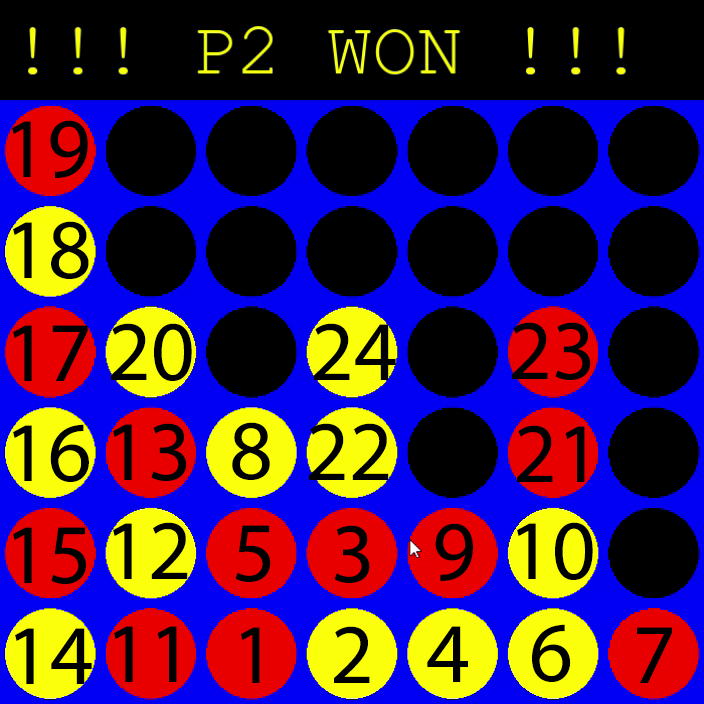
\includegraphics[width=0.7\linewidth]{images/ConnectZero_rainbow_diag_human_win.png}
    \captionsetup{width=0.9\linewidth}
    \captionsetup{justification=centering}
    \caption{Sample connect four game annotated with the time steps at which the coins are placed. Player one is red and is the best-found rainbow policy from the paper notebook 9, player two is yellow and is a human. Player two won with the diagonal coins of 14, 12, 8 and 24.  A video of this game can be found on YouTube (\url{https://youtube.com/shorts/DZesQ4GI0hE}).}
    \label{fig:rainbow_diagonal_win_turn_annotation}
\end{figure}

%------------------------------------

\section{Gym implementation of connect four game environment}
\label{sec:connect_four_rl-gym-environment}


Since this paper aims to study the feasibility of implementing \gls{rl} opponents in simple Python based games, it was chosen to build further upon an existing connect four implementation.
The chosen base implementation is one by \citet{base_connectfour_github} and makes use of the popular Pygame library by \citet{pygame}.
The author's permission of reusing his code was granted after brief communication on LinkedIn.
Some edits were made to this base implementation to make the code more readable and the game UI more informative. 
Since this base game is just a human-play variant of the connect four game, it lacks many of the components required to use it in a \gls{rl} setting such as a reward strategy and more.

As a first step of converting this base Pygame to an environment usable for \gls{marl}, it was converted to a custom Gym environment.
A custom Gym environment should inherit from the Gym class and provide a few specific attributes and functions, a skeleton for this is given in Algorithm \ref{alg:minimal_gym_structure}.
A Gym environment is a class from the popular Gym library by \citet{gym} introduced in section \ref{sec:intro-classical_rl}.
Converting the base Pygame to a Gym environment was straightforward given the many tutorials and documentation available discussing how to create a custom environment.
The conversion process took about four hours, including testing.
This version of the environment is called \texttt{ConnectFourPygameEnvV1} and is available under \texttt{gym\_connect4\_pygame} folder in the Github repository of this project \citep{github_project}. 

The init method supports two render modes, \texttt{terminal} and \texttt{human}.
It also allows for specifying the column and row count of the connect four board, although the default grid of 6x7 is used throughout this paper.
The observation space is specified as a Gym directory consisting of one key called \texttt{board}.
The board in the observation space is a two-dimensional Gym box ($\approx$ 2D array) with integer values between zero and two, including boundaries.
Zero corresponds to an empty space, 1 to the first player's coin and 2 to the second player's coin.
This corresponds to the representation annotated in Figure \ref{fig:intro_rl_cycle}.
The action space is a discrete space specifying an integer that corresponds to the column index a coin should be dropped into.

The step method contains the main logic of a Gym environment as it performs a specified action in the environment and updates the state of the environment.
It also returns a reward, a boolean to specify if the game has ended and an info object.
In this implementation, there is no mechanism in place to reject a player to insert a coin in a full column.
However, attempting to do so keeps the board unaltered and gives the turn to the same player again.
After this, the step function checks for a winning board or tie board to end the game.
If the game is not over, the step function alternates the current player.
The step function makes use of many abstracted functions from the base game, which are not shown in the minimal Gym skeleton of Algorithm \ref{alg:minimal_gym_structure}.

The render method supports a terminal printed render of the board which prints the 2D matrix representation of the board after each step.
It also has support for a human mode which renders the game in a Pygame instance, just like playing the game regularly would do.
The reset and close functions are trivial and are not discussed in detail. 
The experimental notebook 2 gives details on how to work with this V1 of the custom connect four Gym environment \citep{github_project}.
Since the Gym environment doesn't provide any standards on specifying a multi-agent environment, the implementation is custom and does not comply with any specific standard.
In essence, the info object, which is one of the returned values from the step and reset function, gives all the required info for playing a loop in the game.
Since this custom Gym environment is multi-agent but doesn't follow any conventions, it is not supported directly by any \gls{rl} algorithm library and is therefore not used.

\begin{algorithm}
    \caption{Minimal structure of a Gym environment}
    \Comment{Init method should accept a render mode.}
    \Function{\_\_init\_\_(self, render\_mode, ...)}{
        \If{$\var{loss} > \theta_{\mathrm{exp}}$} {
            ... \;
            \Comment{Observation space for the environment: structure of an observation}
            self.observation\_space = gym.spaces.Dict(...)\;
            ...\;
            \Comment{Action space for the environment: structure for an action}
            self.action\_space = gym.spaces.Discrete(...)\;
            ...\;
        }
    }
    \Comment{Reset function to return the environment to its start state.}
    \Function{reset(self, return\_info=False)}{
        ...
        \Return{(observation, info) if return\_info else observation}\;
    }
    \Comment{Step function to perform an action in the environment.}
    \Function{step(self, action: int)}{
        ...\;
        \Comment{Return an observation of the new state, the received reward, a boolean specifying if the environment is finished and an info object containing additional information.}
        \Return{observation, reward, done, info}\;
    }
    \Comment{Render function to visualise the environment.}
    \Function{render(self, mode='terminal')}{
        ...
        
    }
    \Comment{Close function to clean up an environment.}
    \Function{close(self)}{
        ...
    }
    \label{alg:minimal_gym_structure}
\end{algorithm}

%------------------------------------

\section{Petting Zoo implementation of connect four}
\label{sec:connect_four_rl-pettingzoo-environment}

Having implemented the base game as a custom Gym environment in the previous section, it was noted that the Gym library has no direct support or conventions for multi-agent environments.
Because of this, the environment is unlike the other Gym environments, which are all single-agent environments.
This means that it doesn't neatly integrate with existing \gls{rl} algorithm libraries such as Tianshou \citep{tianshou} or Ray RLlib \citep{rllib}.
As this paper is a feasibility study, which includes ease of implementation as a criterion, it was opted to adopt this V1 of the environment to a Petting Zoo environment which is supported by these libraries.
As discussed in section \ref{sec:intro-classical_rl}, Petting Zoo is a commonly used library for \gls{marl} as it provides multi-agent environments in a Gym like fashion.
Converting the custom Gym environment to a Petting Zoo based environment doesn't involve a lot of code changes but did require significant troubleshooting.
This is mostly due to the Petting Zoo documentation not providing instructions on how to implement a custom environment, which the Gym library documentation did do.
However, through studying the source code of simple environments provided by Petting Zoo, such as the Tic-Tac-Toe environment, adopting the custom Gym environment to a Petting Zoo compatible environment took about 15 hours of work.
Most of this time was spent troubleshooting compatibility issues with the Tianshou \gls{rl} algorithm library.

The Petting Zoo variant of the connect four game is provided as \texttt{ConnectFourPygameEnvV2} under the \texttt{gym\_connect4\_pygame} folder in the Github repository of this project \citep{github_project}.  
Most notable changes include inheriting from the Petting Zoo \texttt{AECEnv} class rather than Gym's \texttt{Env} class and wrapping this custom Petting Zoo environment in some common Petting Zoo environment wrappers. 
The observation space is also extended to include an action mask besides the board representation taken straight from the V1 variant of the environment.
This action mask specifies which of the actions from the action space are valid for the current state.
If specified during initialisation, the environment can thus strictly enforce an agent to only use an allowed action for a given state.
Whilst this incorporates some domain knowledge, it can drastically improve the learning speed of the agents.
However, it is still possible to let the agents learn this behaviour by specifying to not use the mask and giving a negative reward for placing a coin in a full column.
Besides this, the observation space and action space should be lists containing a variant of the space for both agents, although these spaces are equal for both agents in the connect four game environment.
Next to this, the \texttt{step} and \texttt{reset} methods no longer return game information such as the state, a done boolean, a reward and an info object.
Rather, Petting Zoo and the libraries that are compatible with it rely on attributes such as \texttt{rewards}, \texttt{dones} and \texttt{infos} to keep track of the game state and an \texttt{observe} function to observe the current state of the environment.
Exact implementation details are not of importance and thus not given in this paper, although the source code is documented and available on GitHub \citep{github_project}.
The final petting zoo environment is over 650 lines of code, compared to the 350 lines of code for the original base game implementation and 450 lines of code for the custom Gym environment (environment V1).  

%------------------------------------

\section{Reward strategy}
\label{sec:connect_four_rl-rewards}

As was discussed in section \ref{sec:marl_opponents}, the target policy of a \gls{marl} problem depends on the reward function, the used discount factor ($\gamma$) and the other agents in the environment.
Whilst the discount factor and agents in the environment can be easily interchanged, the reward strategy has to be implemented in the custom environment.
For the custom Petting Zoo environment, six types of rewards were provided.
The value of each reward can be set during the initialisation of the environment.
The most trivial rewards are those for winning, losing and having a tie game.
To allow for learning not to place a coin in a full column, a (negative) reward for making an invalid move can also be specified.
However, it is noted that the environment can be initialised to use action masks so that the agent can't choose an invalid move, meaning an invalid move would never occur and thus this reward would never be used.

As a means to incentivise longer games, it is also possible to specify a reward for each move made.
Likewise, to incentivise a defensive behaviour by the agent, a reward for what is called a blocking move can also be given.
A move is considered a blocking move if the chosen action by an agent would result in a win for the other agent if the other agent had done that action.
The latter incorporates domain knowledge which guides the agent to learn a good policy.
Whilst this diverges from the purest form of \gls{rl}, it can drastically improve the training time and usability of the policy in terms of human play.
The rewards for making a move and making a blocking move were added incrementally to the environment after it was found that the learned policy using only the other four rewards was very naive.
Chapter \ref{ch:connect_four_eval} discusses the evaluation of the emerged policies and clarifies how different values for these rewards influence the found policies by the agents.


%------------------------------------

\section{Using MLP based deep Q-networks to learn connect four}
\label{sec:connect_four_rl-mlp-dqn}

One of the first very successful \gls{rl} algorithms in learning to play Atari 2600 games at a human level, was a generalisation of the Q-learning algorithm using a \glsfirst{dqn} by \citet{dqn}.
The approach by \citet{dqn} can be seen as a \glsfirst{drl} variant of the popular tabular Q-learning algorithm by \citet{qlearning}.
As discussed in section \ref{sec:intro-approaches}, the difference between tabular methods and \gls{drl} methods is that the first maintains a table of all possible state-action pairs and an expected reward whilst the latter uses \glsfirst{dl} models to map the environment state to an action.
Tabular methods can quickly blow up in dimensionality whilst \gls{drl} can reduce this dimensionality making it possible to solve problems that were not feasible to solve with tabular methods.
As discussed in section \ref{sec:connect_four_rl-harder_then_you_think}, connect four has to many possible states for tabular methods such as Q-learning to be feasible, hence why the \gls{drl} variant \gls{dqn} is used as a first attempt at learning connect four.
More details on how tabular Q-learning works and a convergence proof of the algorithm is given by \citet{qlearning_proof}.

As the name suggests, \gls{dqn} also uses the concept of Q-values just like the Q-learning algorithm but aims to generalise it.
Q-values can be seen as an estimated reward for taking an action ($a$) in a given state ($s$).
These Q-values are the metrics stored in tabular methods for determining and updating the optimal policy.
However, \gls{dqn} doesn't keep track of individual Q-values in a Q-table but rather aims to approximate a Q-function so that the Q-values can be approximated by the Q-function $Q(s, a)$.
In essence, it replaces the Q-table with approximated Q-values in Q-learning by an approximated Q-function.
However, learning that Q-function isn't an easy task, hence why \gls{dl} and more specifically \glspl{ann} come into play.
When using a \gls{dqn}, a \gls{dnn} is used to to approximate the optimal Q-function.

Figure \ref{fig:mlp_dqn} shows one of the \gls{dqn} models that was used for the deep Q-learning of connect four.
This first deep Q-learner is based on a \gls{mlp}.
It consists of three hidden fully connected layers with 128 nodes, all using a ReLu activation function.
The input is the board represented as a 6x7 2D matrix, which corresponds to the state of the environment.
The output is the expected reward for each action if it were taken in that state.
To update this network, a typical loss optimisation is used, in particular, the Adam optimizer proposed by \citet{adam} is used.
The loss function in question is based on the difference in the output of the network with the right-hand side of the Bellman equation given in Equation \ref{eq:bellman}.
Since this target policy makes use of the maximum action $a'$  in the new state $s'$ upon taking an action $a$ in the current state $s$, it differs from the behaviour policy which might use something like epsilon-greedy as well.
Since these two policies are not equal, deep Q-learning is an off-policy approach, just like regular Q-learning, as was discussed in section \ref{sec:intro-approaches}.


\begin{equation}
q_*(s, a) = E[ R_{t+1} + \gamma \max_{a'} q_* (s', a') ]
\label{eq:bellman}
\end{equation}

More technical details on the working of deep Q-learning by using a \gls{dqn} can be found in the paper by \citet{dqn} which first proposed this algorithm.
One of the attractive properties of using the custom Petting Zoo environment is that it directly integrates with the Tianshou library by \citet{tianshou}.
This Tianshou library provides an off-policy learner and a \gls{dqn} policy, which allows for using \gls{dqn} just by specifying which network architecture to use.
This makes the implementation of this rather complex algorithm for our custom connect four Petting Zoo environment extremely simple.
All that has to be done is providing the Pytorch model of the \gls{mlp} based \gls{dqn} shown in Figure \ref{fig:mlp_dqn}.
More implementation details and the chosen parameters for some of Tianshou functions can be found in the paper notebooks 3, 4 and 5 available on the GitHub repository of this project \citep{github_project}.

\begin{figure}[ht]
    \centering
    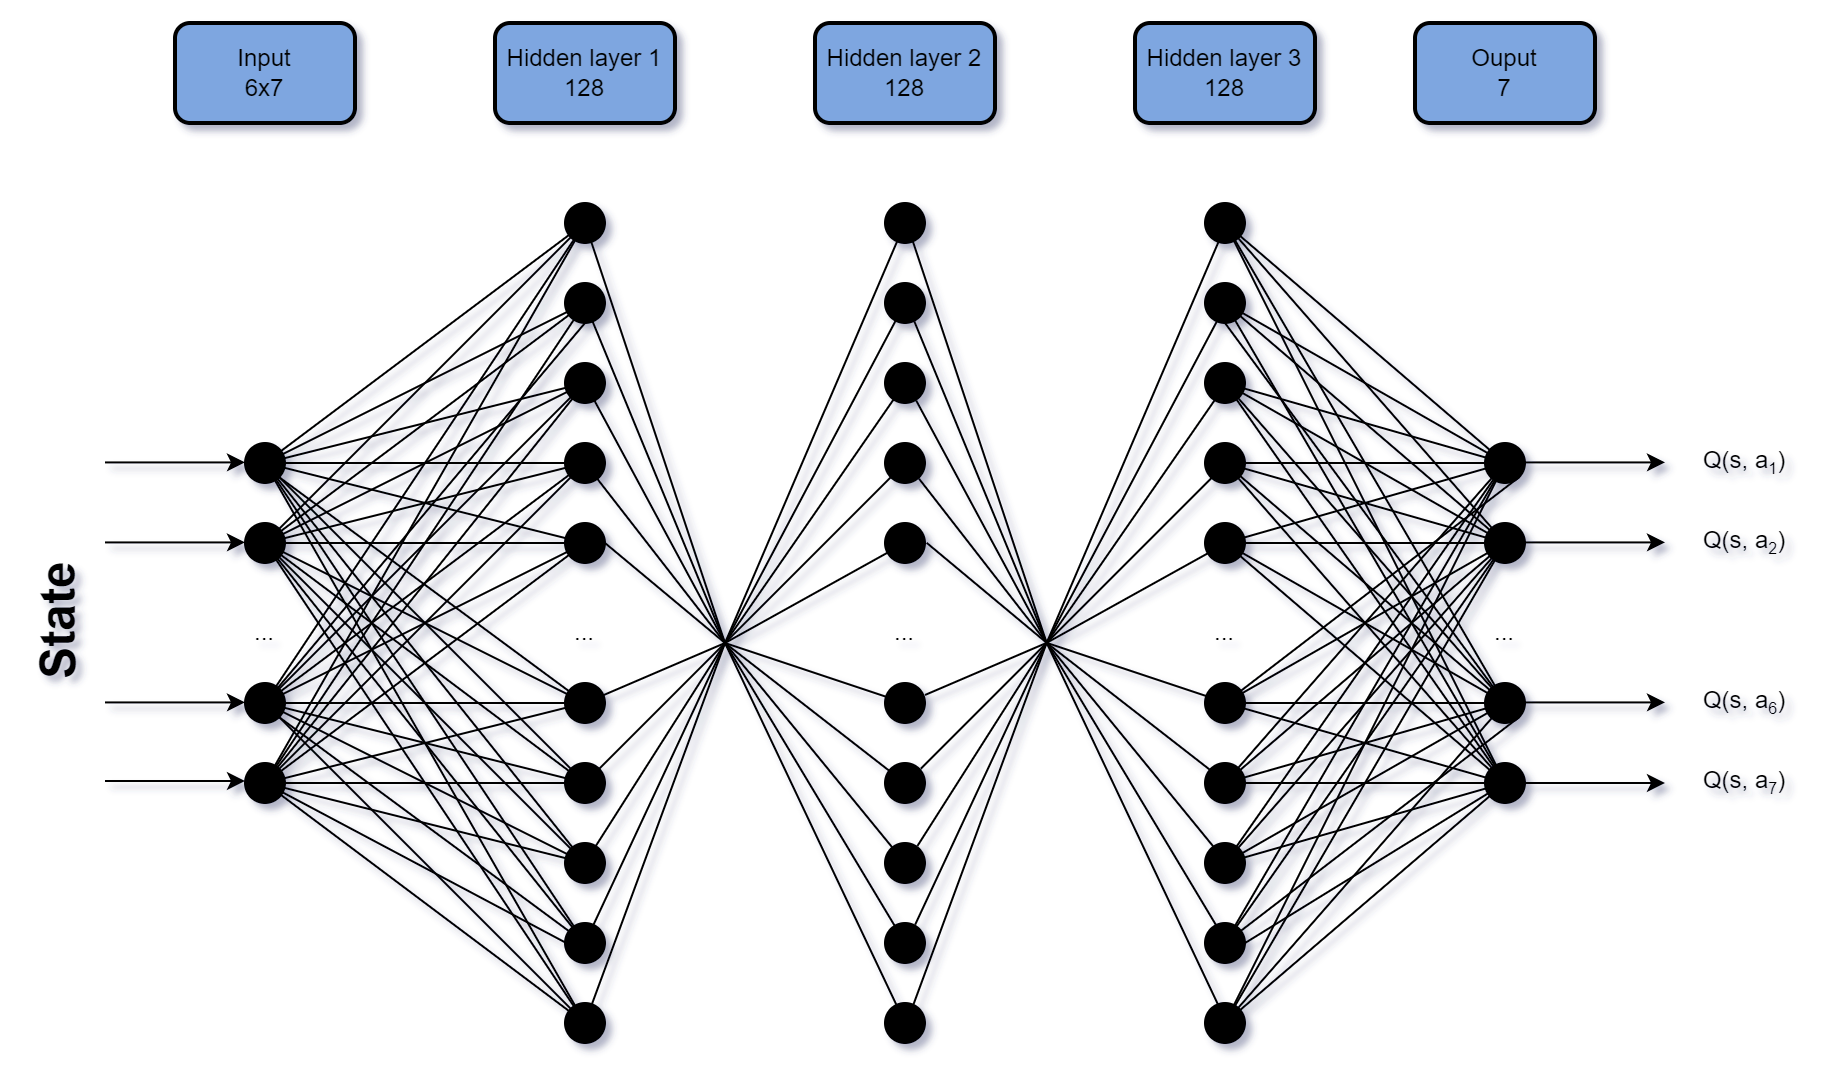
\includegraphics[width=1\linewidth]{images/mlp_dqn.png}
    \captionsetup{width=0.9\linewidth}
    \captionsetup{justification=centering}
    \caption{\gls{mlp} based \gls{dqn} architecture used for Deep Q-Learning.}
    \label{fig:mlp_dqn}
\end{figure}

%------------------------------------

\section{Using CNN based deep Q-networks to learn connect four}
\label{sec:connect_four_rl-cnn-dqn}

The \gls{mlp} based \gls{dqn} proposed in section \ref{sec:connect_four_rl-mlp-dqn} is sophisticated enough that it likely won't be a factor in making learning of the connect four game impossible.
However, there is a more logical architecture to be used.
This more logical architecture revolves around using a convolution layer, forming a type of \gls{cnn}.
Convolution layers are often used for image processing and an in depth explanation of this layer is given by \citet{cnn_explained}.

Intuitively, the 2-dimensional convolutional layer used for the \gls{dqn} goes over the input 2D board representation with a 4x4 kernel.
This kernel consists of a 4x4 grid of weights that have to be learned.
These weights are used to perform a convolution of the 4x4 grid to a singular value.
This kernel moves over the 2D board matrix in a left to right, top to bottom manner, moving by one element each time.
This reduces the initial board input of a 6x7 2d matrix to a 2d matrix of 3x4.
The kernel uses the same weights for the whole board in a single filter.
This process is visualised in Figure \ref{fig:cnn_kernel_explained}.

\begin{figure}[ht]
    \centering
    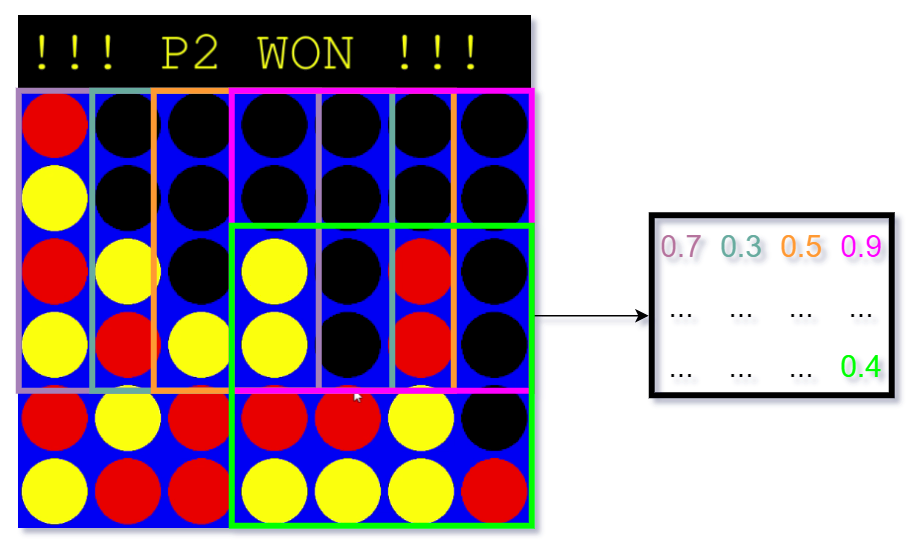
\includegraphics[width=0.7\linewidth]{images/cnn_explained.png}
    \captionsetup{width=0.9\linewidth}
    \captionsetup{justification=centering}
    \caption{Single convolutional filter for a 4x4 kernel with stride one.}
    \label{fig:cnn_kernel_explained}
\end{figure}

Whilst only one such filter would greatly reduce the input dimension, a lot of information would be lost.
At least both diagonal lines, four horizontal lines and four vertical lines should be recognisable since these form a win or a loss condition. 
Whilst it would be possible to learn these conditions with fewer filters, it is reasoned at least 10 or even 20 filters should be available to recognize all win and loss conditions.
Since the computational overhead of providing more filters isn't drastic and it can give better performance by allowing to learn more than just the win conditions, it was opted to create 64 filters.
This results in a final output dimension of 3x4x64 for the convolutional layer.
After this convolutional layer, the output is flattened and two fully connected layers of size 128 are provided before going to the output layer of the network.
In essence, the hidden layer 1 shown in Figure \ref{fig:mlp_dqn} is replaced by 64 filters of the CNN layer visualised in figure \ref{fig:cnn_kernel_explained}.
The implementation of this \gls{cnn} based \gls{dqn} is performed in paper notebook 6 which is available in the GitHub repository of this project \citep{github_project}.


%------------------------------------

\section{Using CNN based Rainbow to learn connect four}
\label{sec:connect_four_rl-rainbow}

Whilst \gls{dqn} has proven to be very powerful at learning single-agent Atari 2600 games, there are some issues with \gls{dqn}.
Many extensions have been proposed to solve one or more of these issues, but they fail to solve all of them or even introduce new ones, as discussed by \citet{rainbow}.
To solve this, \citet{rainbow} proposed a \gls{rl} algorithm that combines all of the strong points of six different \gls{dqn} extensions into a single \gls{rl} algorithm.
This resulted in the best final performance based on the median human-normalized score for 57 Atari 2600 games and required fewer sample frames to do so than any of the individual extensions.
The exact details on the Rainbow algorithm can be found in the \citet{rainbow} paper.
One of the nice things about using the Tianshou library by \citet{tianshou} is the fact that many of these state-of-the-art and complex algorithms are implemented already and can be set up with relatively few lines of code and only a high-level understanding of the algorithm.

The Rainbow algorithm is implemented to use the same convolutional layer of the \gls{cnn} based \gls{dqn} from section \ref{sec:connect_four_rl-cnn-dqn}.
This layer can be seen as a feature extraction layer.
Subsequent layers are adapted from the original Rainbow paper by \citet{rainbow}, where noisy linear layers are used together with an epsilon-decay.
Normally, the algorithm only uses one of these two to make the agents exploratory, but to combat the low amount of training samples due to limited computational power and to incentivise keeping an exploratory behaviour, they are used together for this project.
The rainbow algorithm also makes use of the duelling property described by \citet{dueling} as it should aid in learning a good policy for this \gls{marl} connect four environment.
The implementation of the Rainbow algorithm is further described in the paper notebook 9 on the GitHub repository of this project \citep{github_project}.

%------------------------------------

\section{Using mini-max as a rule-based opponent}
\label{sec:connect_four_rl-minimax_opponent}

Finally, a mini-max based algorithm is implemented to function as a connect four player.
Mini-max is a game tree searching algorithm that can make use of alpha-beta pruning to limit the number of trees to visit.
Intuitively the mini-max algorithm alternates in maximising (current player's optimal strategy) and minimising (opponent's player optimal strategy) the chosen action based on a given score that is returned at the end of the recursive process.
Since it is computationally too hard to do this for the full depth of the game tree, it is only done for a specified depth.
The recursive loop stops once the desired depth is reached or the game is terminated.
When the desired depth is reached, the score of that final state is determined by the number of consecutive coins present on the board for both agents.
If the tree results in a win, the maximum score is returned and if it results in a loss, the minimum score is returned.
A tie is given a score of 0.
Normally, the deeper the search depth, the stronger the policy of the mini-max agent.


However, a mini-max agent does not form a pleasant opponent, since even the simplest mini-max agent with depth 1 will always block a winning move by design.
Thus, to win against the smallest depth mini-max agent, a scenario has to be created where two possible winning moves have emerged.
This ensures that even when the mini-max bot blocks one of them, the game can still be won by playing the other.
This is a rather hard scenario to obtain, and as the depth of the mini-max agent increases, the mini-max agent can anticipate this as well, making it near impossible to beat as a human, even with a depth of only 3.
An ideal bot will sometimes fail to see a potential win for the opponent, as humans would also do.
The mini-max implementation used in this project is based on a mini-max connect four agent by \citet{minimax_base}.
\Citet{minimax_explained} explain the mini-max algorithm in more depth.


Since mini-max uses a fixed policy and doesn't learn from the algorithm, playing against mini-max can be seen as single-agent \gls{rl} as described in section \ref{sec:marl-vs_single}.
However, this mini-max agent has been made available as a Tianshou \texttt{BasePolicy} object so that it can be used in the same multi-agent training pipeline that is used for self-play.
The idea behind playing against a mini-max agent is to provide a strong opponent to learn from for the \gls{rl} agents.
As it is assumed that increasing the depth of the mini-max agent will increase its policy's strength, changing this depth allows for creating a league-based training setting as described in \ref{sec:marl_opponents}.
The best scoring \gls{rl} agent for each of these iterations in the league based training loop would then be incrementally better over the previous iteration.
This would ideally provide varying difficulties for the connect four \gls{rl} bot.
Paper notebook 11 describes this in more depth and is available on the GitHub repository of this project \citep{github_project}.
\chapter{Evaluation of connect four bots}
\label{ch:connect_four_eval}
% experimental results.

%------------------------------------

\section{Objective evaluation of the emerged policies}
\label{sec:connect_four_eval-metrics}
% graph maken van win rate vs random en van player 1 t.o.v. player 2 in self play en van de algs tegen elkaar.

TODO

%------------------------------------

\section{Usability of deep Q-network policy as connect four bot}
\label{sec:connect_four_eval-dqn_vs_human}
% strategies subjective bespreken
% catastrophic forgetting!!!

TODO

%------------------------------------

\section{Usability of Rainbow policy as connect four bot}
\label{sec:connect_four_eval-rainbow_vs_human}
% strategies subjective bespreken

TODO

%------------------------------------

\section{Viability of varying difficulty bot performance}
\label{sec:connect_four_eval-varying_difficulty}
% Minimax uitleggen hoe gebruikt voor moeilijker/makkelijker maar geen statisfactory results deels omdat zo traag is

TODO
\chapter{Discussion}
\label{ch:discussion}

%------------------------------------

\section{Using general purpose libraries for custom tasks}
\label{sec:discussion-library_support}
% Ray RLlib brakka & Tianshou issues but still better then doing it yourself

TODO

%------------------------------------

\section{Reinforcement learning for indie developers}
\label{sec:discussion-rl_for_indie}
% Changes needed especially regarding computational time required but cloud computing maybe solution
% Good school project tho

TODO

%------------------------------------

\section{Takeaways from the experiments}
\label{sec:discussion-takeaways}

TODO

%------------------------------------

\section{Future work}
\label{sec:discussion-future_work}
% Offline learning through human play of your game en uitleggen hoe off policy daarvoor nodig is

TODO

% Glossary
\glsaddall
\printnoidxglossary[type=\acronymtype,title=List of abbreviations and acronyms, nonumberlist, style=listgroup]
\addcontentsline{toc}{chapter}{List of abbreviations and acronyms}

%references list
\nocite{*}
\printbibliography[heading=bibintoc, title={References}]
\end{document}
